
\textbf{Ejemplo 4}\\
Calcular la rentabilidad que gana el inversionista del ejemplo 2 teniendo
en cuenta que la inflación para el año en el que se hizo la inversión fue del
18\% efectivo anual. ¿Cuál es la rentabilidad neta una vez descontada la
retención en la fuente y la inflación?\\ \\
%\newpage %USAR SOLO SI EL SOLUCIÓN QUEDA SOLO Y ES NECESARIO BAJARLO A LA SIGUIENTE PAGINA
\textbf{Solución.}\\
%La tabla ira centrada
\begin{center}
 \renewcommand{\arraystretch}{1.5}% Margenes de las celdas
 %Creación de la cuadricula de 3 columnas
 \begin{longtable}[H]{|c|c|c|}
  %Creamos una linea horizontal
  \hline
  %Definimos el color de la primera fila
  \rowcolor[HTML]{FFB183}
  \multicolumn{3}{|c|}{\cellcolor[HTML]{FFB183}\textbf{1. Asignación período focal}}                                                    \\ \hline
  \multicolumn{3}{|c|}{$pf=1\textit{pav}$}                                                                                            \\ \hline


  %%%%% INICIO DECLARACIÓN DE VARIABLES %%%%%%%
  %%%%%%%%%% INICIO TITULO
  %Lo que se hace aquí es mezclar las 3 columnas en una sola
  \multicolumn{3}{|c|}{\cellcolor[HTML]{FFB183}\textbf{2. Declaración de variables}}                                                  \\ \hline
  %%%%%%%%%% FIN TITULO
  %%%%%%%%%% INICIO DE MATEMÁTICAS
  %Cada & hace referencia al paso de la siguiente columna
  %Cada & hace referencia al paso de la siguiente columna
  \multicolumn{2}{|l|}{ $i = 27,2\% \textit{pav}$ }                                   & $i_{R}=?$                                     \\
  \multicolumn{2}{|l|}{$i_{f} = 18\% \textit{ naav}=18\% \textit{ naav}$  }           &                                               \\
  \multicolumn{2}{|l|}{$i_{f} = \frac{18\%}{1}\textit{naav }=18\%  \textit{naav }$  } &                                               \\ \hline

  %%%%%%%%%% FIN DE MATEMÁTICAS
  %%%%% FIN DECLARACIÓN DE VARIABLES


  %%%%% INICIO FLUJO DE CAJA
  \rowcolor[HTML]{FFB183}
  \multicolumn{3}{|c|}{\cellcolor[HTML]{FFB183}\textbf{3. Diagrama de flujo de caja}}                                                 \\ \hline
  %Mezclamos 3 columnas y pondremos el dibujo
  %%%%%%%%%%%%% INSERCIÓN DE LA IMAGEN
  %Deberán descargar las imágenes respectivas del drive y pegarlas en la carpeta
  %n_capitulo/img/ejemplos/1/capitulo1ejemplo1.pdf  (el /1/ es el numero del ejemplo)
  \multicolumn{3}{|c|}{ 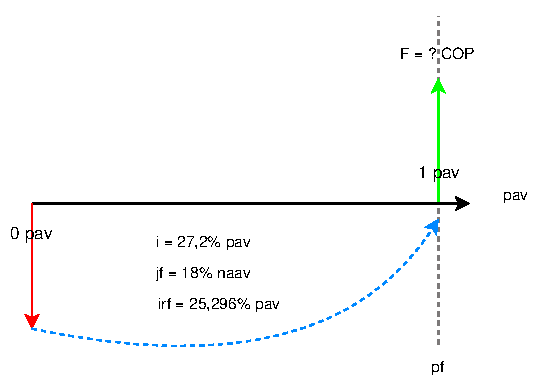
\includegraphics[trim=-78 -5 -78 -5]{3_Capitulo/img/ejemplos/4/capitulo3ejercicio4.pdf} }                                    \\ \hline
  %%%%%%%%%%%%% FIN INSERCIÓN DE IMAGEN
  %%%%%FIN FLUJO DE CAJA



  %%%%% INICIO DECLARACIÓN FORMULAS
  %%%%%%%%%%% INICIO TITULO
  \rowcolor[HTML]{FFB183}
  \multicolumn{3}{|c|}{\cellcolor[HTML]{FFB183}\textbf{4. Declaración de Fórmulas}}                                                   \\ \hline
  %%%%%%%%%%% FIN TITULO
  %%%%%%%%%%% INICIO MATEMÁTICAS

  \multicolumn{3}{|c|}{$i_{R}=\frac{i-i_{f}}{1+i_{f}}$\hspace{2mm} Tasa de interés real }                                             \\ \hline
  %%%%%%%%%% FIN MATEMÁTICAS
  %%%%%% INICIO DESARROLLO MATEMÁTICO
  \rowcolor[HTML]{FFB183}
  %%%%%%%%%%INICIO TITULO
  \multicolumn{3}{|c|}{\cellcolor[HTML]{FFB183}\textbf{5. Desarrollo Matemático}}                                                     \\ \hline
  %%%%%%%%%% FIN TITULO
  %%%%%%%%%% INICIO MATEMÁTICAS
  \multicolumn{3}{|p{\textwidth}|}{$i_{R} =0,272-0,181+0,18= 0,077966 = 7,8\% \textit{ pav}$}                                         \\
  \multicolumn{3}{|p{\textwidth}|}{$i_{R} = \frac{(0,25296 - 0,18)}{(1 + 0,18)} \textit{ Tasa de interes de retencion en la fuente}$} \\
  \multicolumn{3}{|p{\textwidth}|}{$i_{R} = 6,18305085\% \textit{ pav}$}                                                              \\
  \multicolumn{3}{|p{\textwidth}|}{$j_{R} = 6,18305085\% \textit{naav}$}                                                                \\ \hline

  %%%%%%%%%% FIN MATEMÁTICAS
  %%%%%% FIN DESARROLLO MATEMÁTICO


  %%%%%%%%%% FIN MATEMÁTICAS
  %%%%%% FIN RESPUESTA
 \end{longtable}
 %Se crean dos lineas en blanco para que no quede el siguiente texto tan pegado
 %\newline \newline %USARLO SI CREES QUE ES NECESARIO
\end{center}